\chapter{Evaluation}\label{ch:evaluation}

We now evaluate and analyse our designs using a series of different benchmarks and running
the system under different configurations. We run all benchmarks on the
Freescale i.MX 8M Mini quad applications processor with 2GB RAM, running at 1.2 GHz
with a 1Gbps NIC. The configurations for each system tested are specified by each benchmark,
and the system comprises of the following PDs:
\begin{enumerate}
    \item Ethernet Driver
    \item (only as specified) Client Side Ethernet Driver
    \item Rx Mux
    \item Tx Mux: implementation specified in each benchmark
    \item 1 Rx Copy Component per Client application
    \item 1 or more Client applications as specified in each benchmark. 
        The clients use lwIP \cite{Dunkels_01} as an IP stack library for network packet processing. 
    \item (only as specified) Tx Copy Component
\end{enumerate}

For all echo applications, we use ipbench as a distributed load generator 
to send 1472 byte-sized UDP packets to test the seL4 based system. ipbench runs on a 4-node x86 cluster, 
connected to the same switch as our test system,
and counts the number of successful replies from the target system to measure the achieved throughput and latencies.

For all asymmetric client applications, we implement our own custom benchmarking applications to run on an Intel Xeon W-1250
running at 3.3 Ghz, with 64GB RAM and equipped with a 10Gbps NIC. For our transmit-dominant client, our benchmarking
application receives packets using \emph{recv()} and records start and stop time to determine the total transmitted
throughput. For our receive-dominant client, our benchmarking application transmits packets using \emph{send()} and
we count the number of successfully received packets by the client itself to determine the total received throughput.

We also compare some echo server configurations against a Linux system (version 6.1.1) on the same hardware. 
We use a simple user level application which reads and then writes all packets immediately back using the socket API. 
In order to determine the CPU utilisation of both systems, we run an idle thread on each core
at low priority to count the number of idle cycles of that core. 

\section{Asymmetric Client Applications}

Our asymmetric client applications demand significantly more throughput in one direction compared to the 
other. We implement each of the client applications as per \autoref{s:client_apps}.
We measure the total received throughput by a receive-dominant application (Rx Mostly), the
transmitted throughput by a transmit-dominant application (Tx Mostly) and the transmitted throughput
of a client-initiated transmit application (Tx Initiated) and compare these tests against the achieved
throughput of the echo server. 

\begin{figure}[h]
    \centering
    \includegraphics[width=\textwidth]{asym.pdf}
    \caption{Networking Performance of Different Client Applications}
    \label{f:asym}
\end{figure}

\autoref{f:asym} shows the measured throughput as well as the CPU utilisation of each test application. The
receive-dominant application receives over 807Mb/s using 40\% CPU. \TODO{finish this}

\section{Multi-client systems}

Our design has a large number of different paramters to experiment with, including multiplexer
policies, queue sizes and the scheduling parameters of client applications running on the system. 
We select a small variety of example systems to evaluate our different policy designs. We evaluate
these systems with two separate ipbench instances running on different clusters sending UDP packets
at the same time to their respective clients. We split the requested throughput of each client evenly. 

We start first with evaluating single core configurations running two echo server applications. 
Each system comprises of an ethernet driver, Rx Mux, Tx Mux, 2 copy components (1 for Client A, 1 for Client B) 
and two simple echo servers; Client A and Client B. As these systems run on single core, a round robin or priority-based
policy in the Tx Mux would not make sense as the multiplexer runs at higher priority than both the clients and thus
will be invoked as soon as it is signalled by either client. We instead first evaluate a simple Tx Mux that only 
responds to the client that signalled it, and enforce policy through our system design. 

\noindent\begin{figure}[htbp]
    \centering
	\begin{multicols}{2}
		\begin{subfigure}[b]{0.45\textwidth}
        \centering
        \includegraphics[width=1.2\textwidth]{AB.eps}
        \caption{Networking Performance of Two Echo Servers at Equal Priorities}
        \label{f:AB}
    \end{subfigure}\qquad
    \begin{subfigure}[b]{0.45\textwidth}
        \centering
        \includegraphics[width=1.2\textwidth]{AB_RxU16.eps}
        \caption{Networking Performance of Two Echo Servers at Equal Priorities, with limited RxU Queue of Client B}
        \label{f:AB_Rx16}
    \end{subfigure}
\end{multicols}
\end{figure}

\autoref{f:AB} shows the achieved throughput for client A and B and the CPU utilisation of the entire system. 
Both clients are running at equal priority, with their respective copy components at equal, higher priority than their
client, and both clients have a queue size of 512 for all interfacing queues. Both clients achieve the same 
throughput, and their combined total reaches wire speed.\\

We now limit the RxU queue between the Rx Mux and the copy component of client B to just 16 to measure 
the impact this will have on Client Bs throughput. \autoref{f:AB_Rx16} shows the resulting network performance.
Client A still achieves the requested throughput but client B is limited to 400Mbps. This is because the RxU queue
to client B will become full much sooner, causing the Rx Mux to discard subsequent packets for client B and thus
limiting the total throughput available to client B. 

We now incorporate different priorities to our system and measure the impact this has on each clients
achieved performance. We reduce both client B and its copy component to lower priority than client A. 
Thus the priorities are ordered as follows:\\ 

\centerline{Driver \(>\) Tx Mux  \(>\) Rx Mux \(>\) Copier of client A \(>\) Client A \(>\) Copier of client B \(>\) Client B.}

We set all queue sizes to be equal. 

\noindent\begin{figure}[htbp]
    \centering
	\begin{multicols}{2}
		\begin{subfigure}[b]{0.45\textwidth}
        \centering
        \includegraphics[width=1.2\textwidth]{AgtB_RxU32.eps}
        \caption{Throughput Achieved by each Client}
        \label{f:AgtB_RxU32_xput}
    \end{subfigure}\qquad
    \begin{subfigure}[b]{0.45\textwidth}
        \vspace{39pt}
        \centering
        \includegraphics[width=1.2\textwidth]{AgtB_RxU32_latency.eps}
        \caption{Median Latencies for each Client}
        \label{f:AgtB_RxU32_latency}
    \end{subfigure}
\end{multicols}
\caption{Networking Performance of Two Echo Servers at Different Priorities}
\label{f:AgtB_RxU32}
\end{figure}

We see in \autoref{f:AgtB_RxU32_xput} the throughput of the lower priority client remains unaffected as there isn't enough
contention on the CPU to limit this clients CPU bandwidth and both clients achieve their requested load.
However, the latencies are affected by this. \autoref{f:AgtB_RxU32_latency} shows the median round trip time (RTT)
for each client from a sample size of 200,000 packets. Client A achieves lower latencies than client B as it is running
at higher priority and thus is scheduled to run first.

If there was more contention for the CPU, then we would expect the priority assignment of each client to have an effect
on their achieved throughput. We now add unnecessary overhead to each packets round trip to simulate an environment where
this is the case. We have each client copy each packet and calculate a checksum 10 times as per \autoref{s:compute_heavy}. 

\noindent\begin{figure}[h]
    \centering
	\begin{multicols}{2}
		\begin{subfigure}[b]{0.45\textwidth}
        \centering
        \includegraphics[width=1.2\textwidth]{AgtB_overload.eps}
        \caption{Equal Queue Sizes}
        \label{f:AgtB_overload}
    \end{subfigure}\qquad
    \begin{subfigure}[b]{0.45\textwidth}
        \centering
        \includegraphics[width=1.2\textwidth]{AgtB_RxU32_overload.eps}
        \caption{Limit RxU Queue of Client B to 32}
        \label{f:AgtB_RxU32_overload}
    \end{subfigure}
\end{multicols}
\caption{Networking Performance of Two Overloaded Echo Servers at Different Priorities}
\label{f:AgtB_od}
\end{figure}

\autoref{f:AgtB_overload} shows the achieved throughput for both clients. Neither client achieves its requested load, with client A,
the higher priority client, maxing out at 400Mbps and client B seeing a performance collapse to 300Mbps. By the total achieved throughput
and CPU load, it is clear the system is overloaded at this point. However, it is clear that client B as the low priority client is 
starving client A by monopolising shared Rx buffers, as client A is not able to achieve its requested load. We now limit client Bs RxU queue
to 32, to prevent this and ensure there are adequate Rx buffers available to higher priority clients as per \autoref{s:rx_policy}. 
\autoref{f:AgtB_RxU32_overload} shows the resulting performance. The total throughput achieved is not affected by this change, and the
system still becomes overloaded at 400Mbps. However, client A is now able to achieve its requested load as client Bs available
Rx throughput is limited. \\

The results all indicate that limiting a clients queues limits its available throughput. We can use this property to implement 
a bandwidth-limited policy in the system. We now limit the RxU queue between the Mux and Copier of client B to just 16, and also
limit the TxU queue between the Mux and client B. Client B and its Copier still run at lower priority than Client A, and both
clients are just simple echo servers (with no additional overload).

\begin{figure}[h]
    \centering
    \includegraphics[width=7cm]{AgtB_RxTxU16.eps}
    \caption{Networking Performance of Two Echo Servers with Limited Queues to Client B}
    \label{f:AgtB_RxTxU16}
\end{figure}

\autoref{f:AgtB_RxTxU16} shows the resulting performance. Client A still achieves its requested load, but client B is limited
to just 200Mbps. The total CPU load is also reduced compared to the system without any queue limits, indicating less load on 
the limited client.

\subsection{Bandwidth-limited Tx Multiplexer}

We can also limit clients available bandwidth using policy in the Tx Mux. We evaluate \autoref{s:bandwidth} with two echo servers,
running at equal priority and with equal queue sizes, and limit client B to just 100Mbps in the Tx Mux. 

\begin{figure}[h]
    \centering
    \includegraphics[width=7cm]{Tx_Limited.eps}
    \caption{Networking Performance of Two Echo Servers with Limited Bandwidth}
    \label{f:Tx_Limited}
\end{figure}

\autoref{f:Tx_Limited} shows the achieved throughput for both clients and the total CPU load of the system. As expected, client A which
does not have a bandwidth limit, achieves its requested load and client B is limited to just 100Mbps. 

\section{Multicore}

% Non, single core SMP vs Two Cores. 
% Comparisson against linux
\begin{figure}[h]
    \centering
    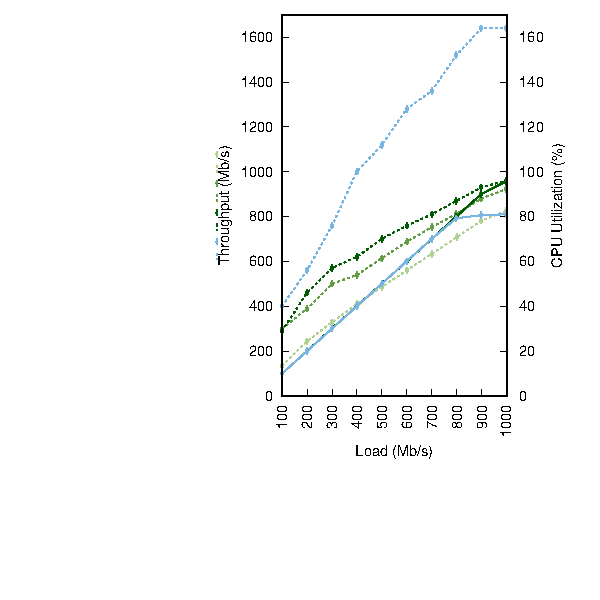
\includegraphics[width=\textwidth]{multicore.pdf}
    \caption{Networking Performance comparisson}
    \label{f:multicore}
\end{figure}



% muxes 
\subsection{Round Robin Tx Multiplexer}

\begin{figure}[h]
    \centering
    \includegraphics[width=10cm]{Tx_Round_Robin.eps}
    \caption{Networking Performance of Two Echo Servers with Round Robin Multiplexer}
    \label{f:round_robin_mux}
\end{figure}

\subsection{Priority-based Tx Multiplexer}

\begin{figure}[h]
    \centering
    \includegraphics[width=10cm]{Tx_Priority.eps}
    \caption{Networking Performance of Two Echo Servers with Priority-based Multiplexer}
    \label{f:priority_mux}
\end{figure}

\begin{figure}[h]
    \centering
    \includegraphics[width=10cm]{Tx_Priority_latency.eps}
    \caption{Networking Latencies of Two Echo Servers at with Priority-based Multiplexer}
    \label{f:priority_latency}
\end{figure}

\subsection{Core allocation}

\begin{figure}[h]
    \centering
    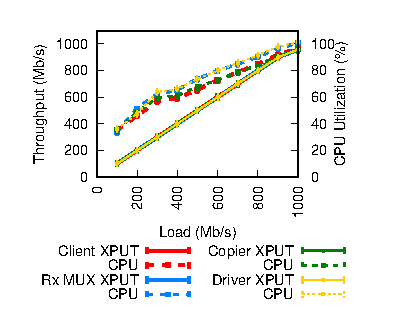
\includegraphics[width=10cm]{multicore_distr.eps}
    \caption{CPU Utilisation with Select Components Isolated on a Separate Core}
    \label{f:multicore_distr}
\end{figure}

\subsection{Two Threaded Driver}

\begin{figure}[h]
    \centering
    \includegraphics[width=10cm]{2driver_comp.eps}
    \caption{Performance Comparisson of Two Threaded Driver on Multi-core}
    \label{f:2driver_comp}
\end{figure}

\begin{figure}[h]
    \centering
    \includegraphics[width=10cm]{multicore_overload.eps}
    \caption{Networking Performance with 4 Clients on Multi-core}
    \label{f:multicore_overload}
\end{figure}

\begin{figure}[h]
    \centering
    \includegraphics[width=10cm]{2driver_comp_overload.eps}
    \caption{Performance Comparisson of Two Threaded Driver with 4 Clients on Multi-core}
    \label{f:2driver_comp_overload}
\end{figure}

\begin{figure}[h]
    \centering
    \includegraphics[width=10cm]{core_analysis_multicore_overload.eps}
    \caption{Core Utilisation of 4 Clients on Multi-core}
    \label{f:core_analysis_mutlicore_overload}
\end{figure}

\begin{figure}[h]
    \centering
    \includegraphics[width=10cm]{core_analysis_multicore_overload_2driver.eps}
    \caption{Core Utilisation of Two Threaded Driver with 4 Clients on Multi-core}
    \label{f:core_analysis_mutlicore_overload_2driver}
\end{figure}

\section{Transmit Copy Component}

\begin{figure}[h]
    \centering
    \includegraphics[width=10cm]{tx_copy_overhead.eps}
    \caption{Performance Overhead with Tx Copy Component}
    \label{f:tx_copy_overhead}
\end{figure}
